% !TEX TS-program = lualatex
% !TEX encoding = UTF-8

% This is a simple template for a LuaLaTeX document using gregorio scores.

\documentclass[letterpaper,12pt]{book} % use larger type; default would be 10pt

\input{header.inc}

\geometry{letterpaper,outer=0.9in,inner=0.4in,top=1in,bottom=0.8in}

\begin{document}

{
	\garamondbig
	\greannotation{Hymn.}
	\greannotation{4.}
	\gregorioscore{210_hy--creator_alme_siderum--solesmes}

	\bigskip

	\Vbar{}.~Roráte cǽli désuper, et núbes plúant jústum.

	\Rbar{}.~Aperiátur térra, et gérminet Salvatórem.

	\bigskip

\begin{centering}

\vfill

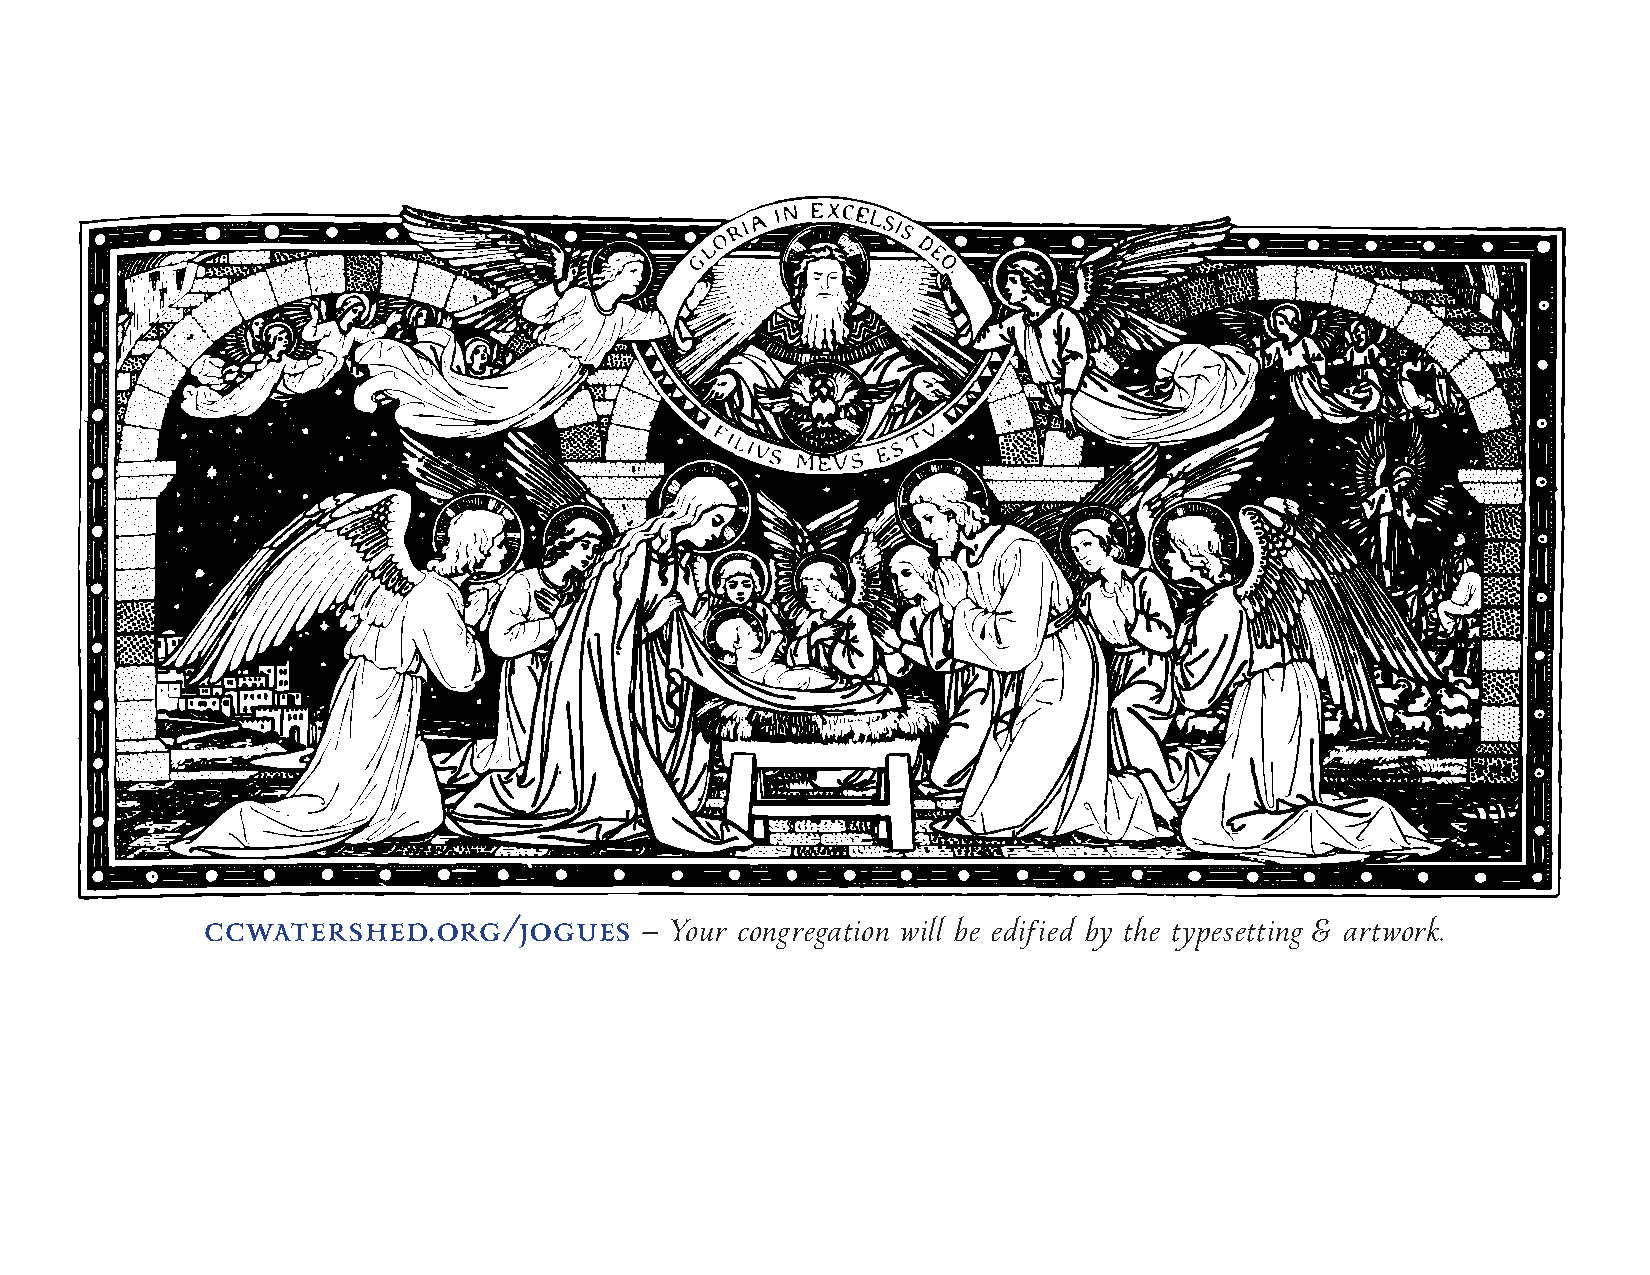
\includegraphics[clip,trim=0.5in 2.494in 0.5in 1.26in,width=\textwidth]{../211_clipart.pdf}

\vfill

\end{centering}

	\greannotation{1.}
	\gregorioscore{212_va--rorate_caeli--solesmes.1}

	{\it The Choir repeats~:} Roráte.

	\garamondbig
	\gresetinitiallines{0}
	\gregorioscore{212_va--rorate_caeli--solesmes.2}

	\Rbar.~Roráte.

	\bigskip

	\gresetinitiallines{0}
	\gregorioscore{212_va--rorate_caeli--solesmes.3}

	\Rbar.~Roráte.

	\bigskip

	\gresetinitiallines{0}
	\gregorioscore{212_va--rorate_caeli--solesmes.4}

	\Rbar.~Roráte.

	\bigskip

	\gresetinitiallines{0}
	\gregorioscore{212_va--rorate_caeli--solesmes.5}

	\Rbar.~Roráte.
}

\bigskip
\pagebreak

\printsmalltitle{Christmas Vesper Hymn}

{
	\garamondbig
	\gresetinitiallines{1}
	\greannotation{Hymn.}
	\greannotation{1.}
	\gregorioscore{215_hy--jesu_redemptor_omnium--solesmes}

	\gresetinitiallines{0}
	\gregorioscore{217_vr_crastina}
}

\bigskip

\begin{centering}

\vfill

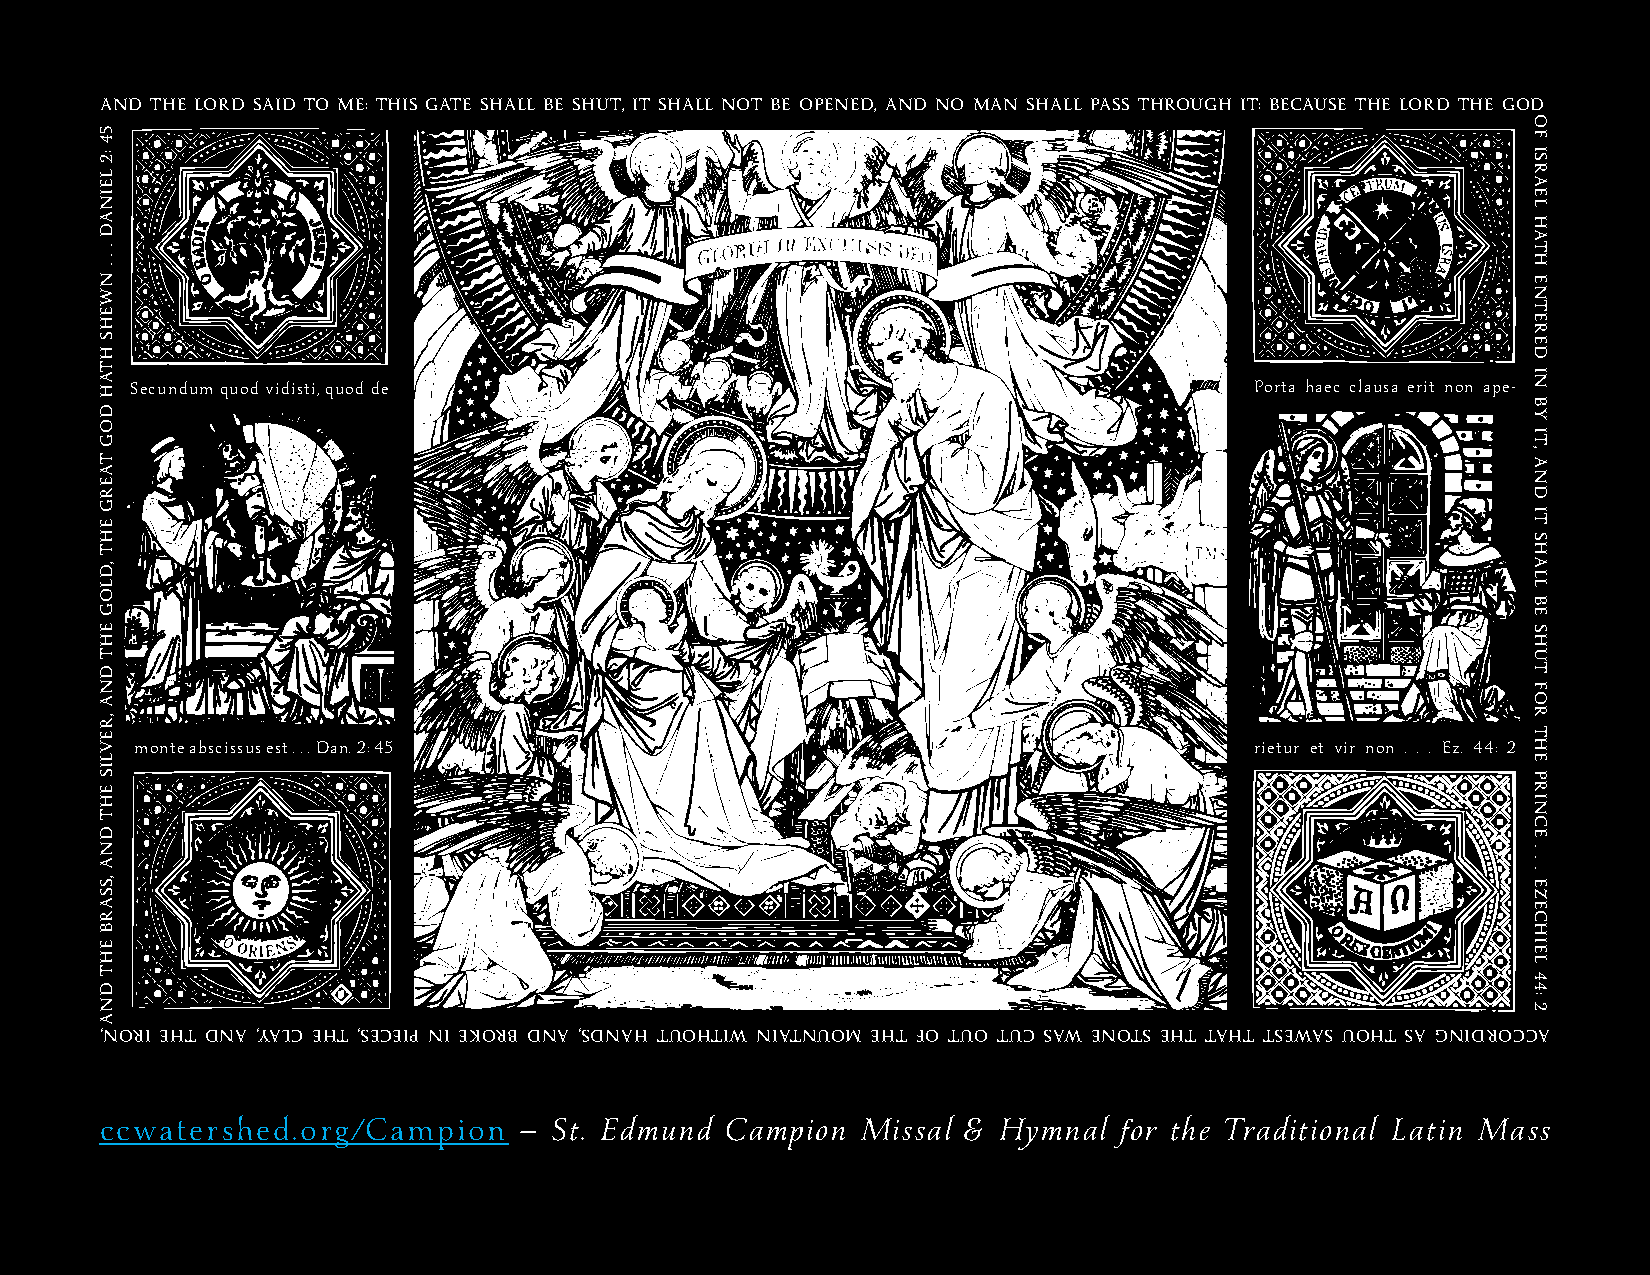
\includegraphics[clip,trim=2.755in 1.773in 2.826in 0.856in,width=0.85\textwidth]{../217_clipart.pdf}

\vfill

\end{centering}


\printsmalltitle{Holy Name Vesper Hymn}

{
	\garamondbig
	\gresetinitiallines{1}
	\greannotation{Hymn.}
	\greannotation{1.}
	\gregorioscore{218_hy--jesu_dulcis_memoria--solesmes}
}

\bigskip

\printsmalltitle{Iesu Dulcis Amor}

{
	\garamondbig
	\greannotation{Cant.}
	\greannotation{1.}
	\gregorioscore{219_ca--jesu_dulcis_amor--solesmes}
}

\bigskip
\pagebreak

\printsmalltitle{Epiphany Vesper Hymn}

{
	\garamondbig
	\greannotation{Hymn.}
	\greannotation{3.}
	\gregorioscore{221_hy--crudelis_herodes_deum--solesmes}
}

\bigskip
\begin{centering}

\vfill

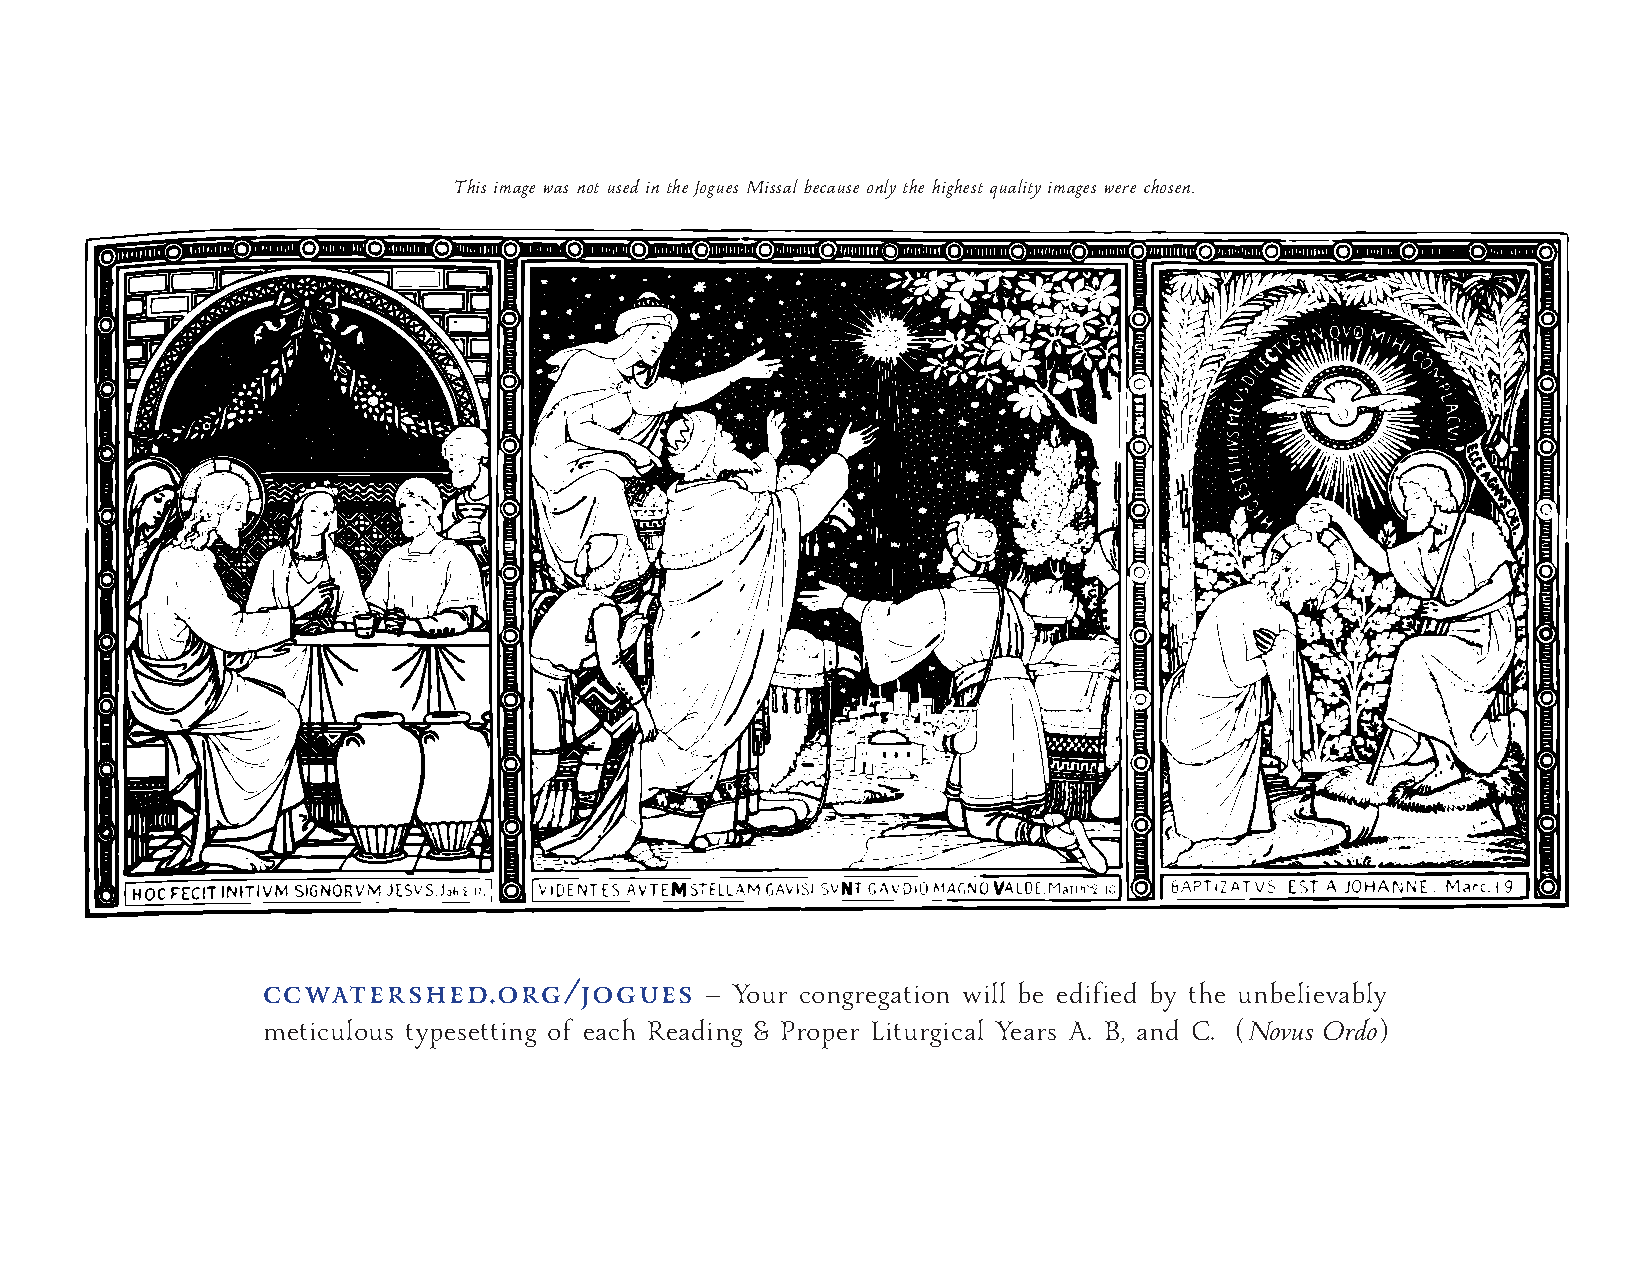
\includegraphics[clip,trim=0.5in 2.317in 0.5in 1.47in,width=\textwidth]{../222_clipart.pdf}

\vfill

\end{centering}
\pagebreak

\printsmalltitle{Another version}

{
	\garamondbig
	\greannotation{Hymn.}
	\greannotation{8.}
	\gregorioscore{223_hy--crudelis_herodes_deum_another_chant--solesmes}
}

\bigskip

\begin{centering}

\vfill

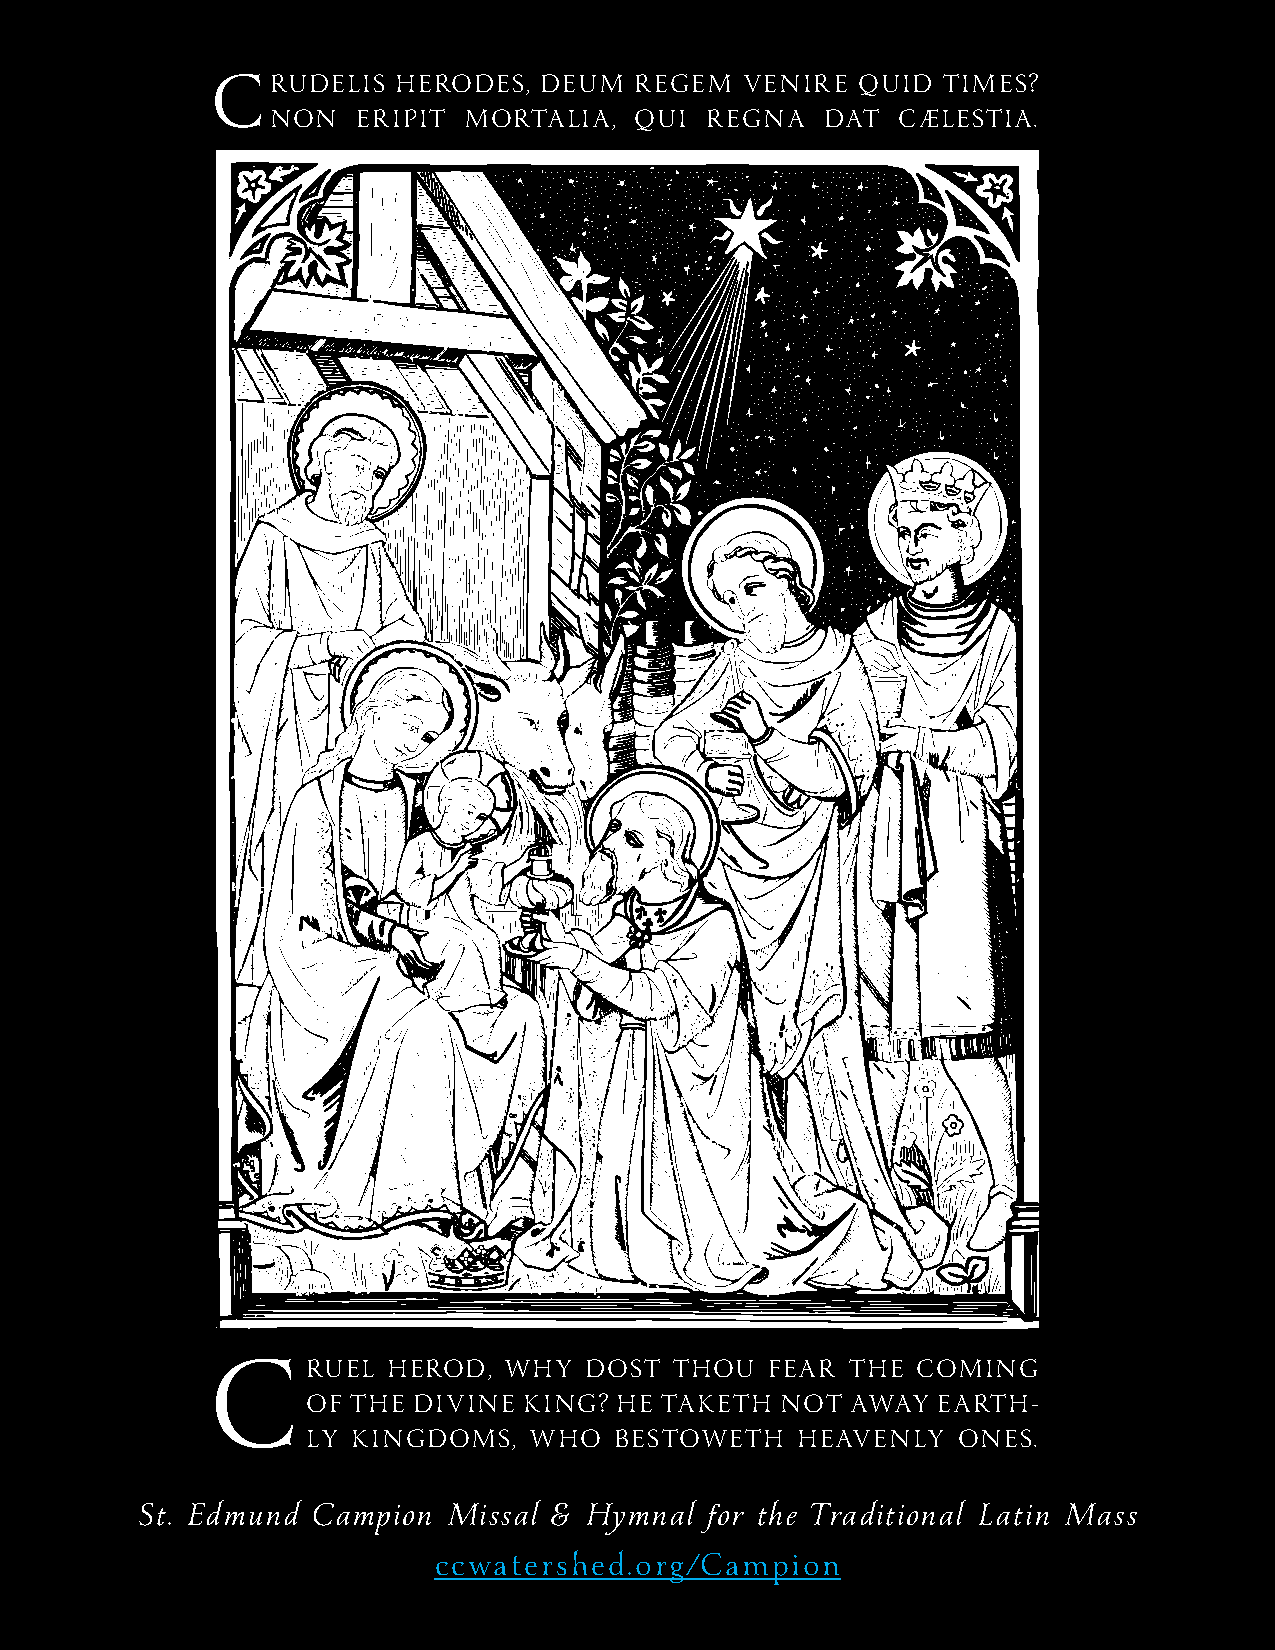
\includegraphics[clip,trim=1.445in 2.141in 1.577in 1.005in,width=0.64\textwidth]{../224_clipart.pdf}

\vfill

\end{centering}
\pagebreak

\printsmalltitle{Holy Family Vesper Hymn}

{
	\garamondbig
	\greannotation{Hymn.}
	\greannotation{2.}
	\gregorioscore{225_hy--o_lux_beata--solesmes}
}

\bigskip





\end{document}